\documentclass[a4paper]{article}

\usepackage{fullpage}
\usepackage{amsmath}
\usepackage{amssymb}
\usepackage{listings}
\usepackage{parcolumns}
\usepackage{graphicx}

\title{An instantiation algorithm for TLA+ expressions}

\newcommand{\assignment}[1]{\{#1\}}
\newcommand{\inst}[2]{#1 {\leftarrow} #2}
\newcommand{\einst}[3]{#1 \stackrel{#2}{\Leftarrow} #3}
\newcommand{\tlaplus}[0]{{TLA+}}
\newcommand{\tla}[1]{#1}

\newcommand{\dor}{\textbf{or}}

\newcommand{\sidebyside}[2]{
    \begin{minipage}{0.45\linewidth}
      #1
    \end{minipage}
    \space{10pt}
    \begin{minipage}{0.45\linewidth}
      #2
    \end{minipage}
}

\lstdefinelanguage{tlaplus}{
  morekeywords= { MODULE, LET, IN, VARIABLE, VARIABLES, CONSTANT, CONSTANTS,
    ASSUME, NEW, PROVE, THEOREM, LEMMA, ENABLED, ==, INSTANCE, BY, DEF },
  sensitive=true,
  morecomment=[l]{\*},
  morecomment=[s]{(*}{*)},
  morestring=[b]",
  literate={~} {$\sim$}{1},
  columns=fullflexible,
  basicstyle=\small
}

\lstset{language=tlaplus}

\begin{document}

\maketitle

\section{Overview}
\label{sec:overview}
\tlaplus{} has two kinds of substitution: instantiation of modules, which
 preserves validity, and beta-reduction of lambda-expressions, which does not
 necessarily preserve validity. Moreover, the two substitutions do not commute.
 For example, let us consider modules Foo and Bar:

\begin{parcolumns}{2}
\colchunk{
\begin{lstlisting}
---- MODULE Foo ----

VARIABLE x

E(u) == x' # u'
D(u) == ENABLED ( E(u) )

THEOREM T1 == ~ D(x)

====
\end{lstlisting}
}
\colchunk{
\begin{lstlisting}
---- MODULE Bar ----

VARIABLE y

I == INSTANCE Foo with x <- y


THEOREM T2 == D(y)

====
\end{lstlisting}
}
\end{parcolumns}

\vspace{2mm}
\noindent
It looks like \tla{I!T1} and \tla{T2} talk about the same formula \tla{D(y)},
 but this is not the case: the first can be read as \tla{I!(D(y))}\footnote{This
 is not valid \tlaplus{} syntax.} and the second as \tla{(I!D)(y)}. In other
 words, it makes a difference if we beta-reduce first or if we instantiate
 first. Reducing D(x) first leads to \tla{ENABLED (x' \# x')}, which -- following the
 renaming instuctions in ``Specifying Systems'' -- becomes \tla{ENABLED (\$x'
 \# \$x')} by the instantiation of \tla{x} with \tla{y}, where primed
 occurrences of \tla{\$x} are bound by their enclosing ENABLED and therefore
 untouched.

Instantiating first keeps the occurrence of the  variable \tla{u} intact,
 leading to \tla{I!D(u) == ENABLED ( u \# \$x') }. Unfolding the definitions and
 reducing the application \tla{I!D(y)} subsequently leads to
 \tla{ENABLED (y' \# \$x')}. Now it is clear that \tla{I!(D(y))} is
 unsatisfiable while \tla{(I!D)(y)} is satisfiable. Since \tlaplus{}
 contains set theory, finite domains -- and in particular, single element
 domains -- are excluded. Therefore \tla{(I!D)(y)} is a theorem in \tlaplus{}.

In the following, we will develop algorithms for both kinds of substitutions.
 Since inner substitutions have to be carried out before applying outer ones,
 special consideration will be taken with regard to partially unfolded
 definitions.

\section{New Attempt: Explicit subtitutions}

The original idea here is to represent both beta-reduction and instantiation
 explicitly in the term graph. Then the two formulas in the introduction
 could be written as D(u)\{u $\mapsto$ x\}[x $\mapsto$ y] and
 D(u)[x $\mapsto$ y]\{u $\mapsto$ x\}, where reduction is denoted by curly
 braces and instantiation is denoted by square braces. Actually, the SANY
 data-structures allow to write reduction as application to an abstraction:
 D(u)\{u $\mapsto$ x\} is then just \tla{(LAMBDA u: D(u))(x)}. Again, this
 is not legal \tlaplus{} but allowed by SANY.


\subsection{Datastructures}
\label{sec:ds}

\begin{tabular}{lll}
node & content & comment \\
\hline
Module & list of constants, list of variables, & \\
       & list of instances, list of definitions & \\
Constant  & name, arity & Set of Constants CS \\
Variable  & name & arity == 0, Set of Variables VS \\
Parameter & name, arity & Set of Paramters FP \\
Definition & name, arity, list of parameters, expression body & Set of Definitions DS\\
Expression  & constant & \\
          & \dor{} variable & \\
          & \dor{} parameter & \\
          & \dor{} definition & \\
          & \dor{} abstraction &\\
          & \dor{} application &\\
          & \dor{} substin & \\
%          & \dor{} selector &\\
Application & head expression, argument expression list & head.arity == list length\\
Abstraction & parameter, expression body & \\
SubstIn     & instantiation, expression body & the explicit instantiation node \\
Instance & module, parameters, instantiation & \\
Instantiation & list of assigments of variables/constants to expressions& \\
%Selector & instance, definition & the ! operator\\
\end{tabular}

The definition and instantiation elements do not contain arguments since they
 can always be rewritten in terms of abstractions: D(x) == F is equivalent to
 D == LAMBDA x : F and I(x)!D is equivalent to LAMBDA x : I!D. We write
 abstraction as $\lambda x : F$ and instantiation as $(\rho M\; with x_1
 \leftarrow t_1,\ldots,x_n \leftarrow t_n)!e$ where the variables / constants
 $x_i$ are exactly those declared in the module $M$.

We assume we have a set $Unfolded$ of definitions which are unfolded and
 a context tracing if we are inside ENABLED.

Rewrite rules:\\

\[
\begin{array}{l@{\;\;\rightarrow\;\;}lll}
  (\lambda x : c)(e) &  c & c \in CS \cup VS & \\
  (\lambda x : x)(e) &  e & x \in FP &\\
  (\lambda x : y)(e) &  y & y \in FP&\\
  (\lambda x : D)(e) &  (\lambda x : b)(e) & D \in DS, b = D.body,
                                             D \in Unfolded&\\
  (\lambda x : f(g))(e) & ((\lambda x : f)(e))(\lambda x : g)(e)) &\\
  (\lambda x : \lambda y : s)(t)
                     & (\lambda y : (\lambda x : s)(t))
                          & y \not \in FV(s) \cup FV(t) & ***\\
  (\lambda x : \lambda y : s)(t)
                     & (\lambda x : (\lambda z : (\lambda y : s)(z))(t))
                          & y \in FV(s) \cup FV(t) , \\
  \multicolumn{2}{l}{} & z \not \in FV(s) \cup FV(t) & \\
  \hline
  (\rho M\; with\; c \leftarrow s)! x & s & c \in CS \cup VS & * \\
  (\rho M\; with\; c \leftarrow s)! x & x & x \in FP &\\
  (\rho M\; with\; c \leftarrow s)!D & (\rho M\; with\; c \leftarrow s)!(b)
                          & D\in DS, D \in Unfolded, b = D.body&\\
  (\rho M\; with\; c \leftarrow s)!(f(g))
                     & (\rho M\; with\; c \leftarrow s)!(f)
                       ((\rho M\; with\; c \leftarrow s)!(g) ) & f \neq '\mbox{ or }f\mbox{ outside of }EN  &\\
  (\rho M\; with\; c \leftarrow s)!(g')
                     & ((\rho M\; with\; c \leftarrow \$c)!(g) )' & '\mbox{ inside of }EN, \$c \not \in CS\cup VS  &**\\
\end{array}
\]

Remarks:\\
\begin{tabular}{ll}
  * & all modules of M are instantiated \\
  ** & this is unclean since it doesn't capture the difference between \\
     &  $EN (x\neq x' \land x=x')$ and $EN (x\neq x') \land EN (x=x')$ well\\
  \\
  & FP-substitution stops at folded definitions and CS/VS subtitutions\\
  & CS/VS-substitution stops at folded definitions and FP-substitutions\\
\end{tabular}


\subsection{Termination}
\label{sec:termination}

We define a lexicographic order on the following measures:

\begin{enumerate}
\item Variable name clashes:
  \begin{itemize}
  \item $clash(c)=clash(v)=clash(fp)=0$
  \item $clash(s(t)) = clash(s) + clash(t)$ where $s$ is not abstraction
  \item $clash(\lambda x . s) t = clash(s)$ if $x \not \in FV(t)$
  \item $clash(\lambda x . s) t = clash(s) + 1$ if $x \in FV(t)$
  \item $clash(\lambda x . s) = clash(s)$ for the cases not covered above
  \end{itemize}

% \item Number of applications inside abstractions:
%   \begin{itemize}
%   \item $apps(c)=apps(v)=apps(fp)=0$
%   \item $apps(s(t)) = 1 + apps(s) + apps(t)$
%   \item $apps(\lambda x . t) = apps(t)$
% 
%   \item $absapps(c)=absapps(v)=absapps(fp)=0$
%   \item $absapps(s(t)) = absapps(s) + absapps(t)$
%   \item $absapps(\lambda x . t) = apps(t)+absapps(t)$
%  \end{itemize}

  
\item Deepest term under an abstraction which can be applied:
  \begin{itemize}
  \item $d(v)=d(c)=d(fp)=0$
  \item $d(\lambda x . s)=1 + d(s)$
  \item $d(s(t))= 1 + max(d(s), d(t))$
  \end{itemize}

  \begin{itemize}
  \item $da(v)=da(c)=da(fp)=0$
  \item $da(\lambda x . s)=1 + da(s)$
  \item $da(s(t))= \left\{
      \begin{array}{rl}
        1 + d(s) + max(da(s),da(t))&\mbox{if }s=\lambda x.r\\
        max(da(s),da(t))&\mbox{otherwise}\\
      \end{array}\right.$
  \end{itemize}

\end{enumerate}

\section{Open Problems}
\begin{itemize}
\item Confluence: I only checked overlaps of root position vs root position,
  non-root overlaps are possible
\item The ordering $da$ does not decrease in some cases (e.g.: wrap the redex of
  the *** rule into an application redex(e)). The reason is that outer pattern
  matches weigh heavier than inner ones:
  \begin{center}
    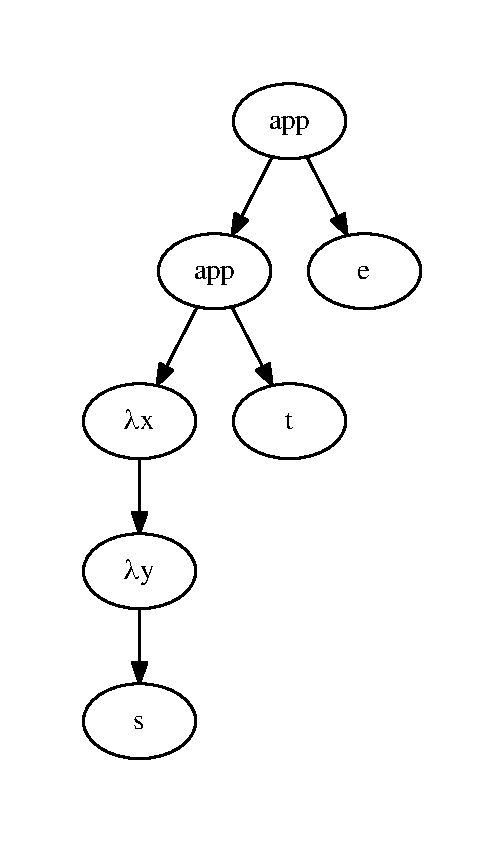
\includegraphics[width=4cm]{measure_ce1.pdf}
    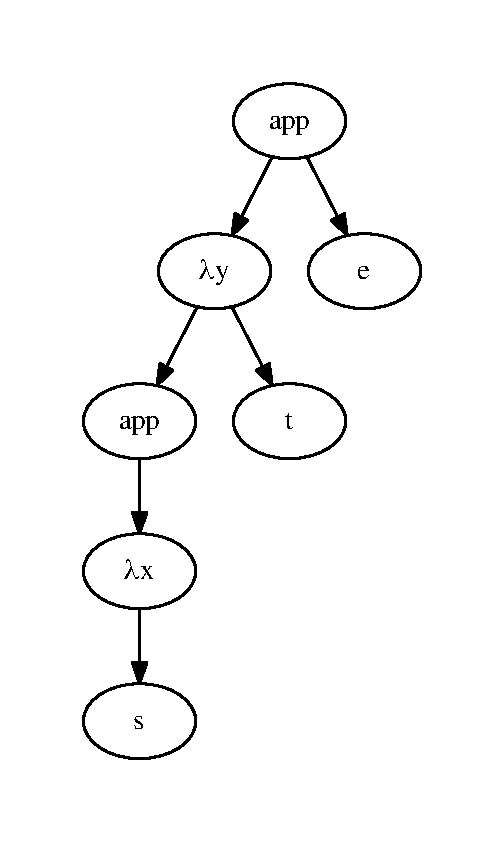
\includegraphics[width=4cm]{measure_ce2.pdf}
  \end{center}
\end{itemize}

The weight of the abstraction on $x$ decreases as expected, but at the same time
 the weight of the abstraction on $y$ increases. Since $y$ is higher, its weight
 contributes more.

\section{Excursion: parametrized instantiations in SANY}
\label{sec:param-inst}

In SANY, parametrized instantuitions have a representation where the
 parameter is shifted over the instantiation. Let us consider the
 modules Foo and Bar:

\begin{parcolumns}{2}
\colchunk{
  \begin{lstlisting}
---- MODULE Foo ----

 VARIABLE a

 D(u) == u' # a'
 E(u) == D(u) \/ ENABLED D(u)

====
    \end{lstlisting}
}
\colchunk{
  \begin{lstlisting}
---- MODULE Bar ----
 EXTENDS Naturals

 VARIABLE x

 I(v) == INSTANCE Foo WITH a <- x+v

====
  \end{lstlisting}
}
\end{parcolumns}

The term \tla{I(x)!E(x)} is represented as \tla{I!E(x,x)} but they are
 not equivalent. In the meta-notation, they would be
 E\{u $\mapsto$ x\}[a $\mapsto$ x+v]\{v $\mapsto$ x\} vs. E\{u $\mapsto$ x,
 v $\mapsto$ x\}[a $\mapsto$ x+v] with the same consequences as in the
 introduction.


TODOs:\\
\begin{itemize}
\item  compute the set of unfolded defs
\item  $(ENABLED\; A) \Leftrightarrow  C$ used instantiated
\end{itemize}
\end{document}
